% !TEX program = xelatex
\documentclass[12pt,a4paper]{article}

\usepackage[a4paper,margin=2.4cm,headheight=16pt]{geometry}
\usepackage{fontspec}
\usepackage[brazil]{babel}
\usepackage{graphicx}
\usepackage{float}
\usepackage{booktabs}
\usepackage{tabularx}
\usepackage{array}
\usepackage{xcolor}
\usepackage{hyperref}
\usepackage{caption}
\usepackage{subcaption}
\usepackage{enumitem}
\usepackage{titlesec}
\usepackage{fancyhdr}
\usepackage{lastpage}

\setmainfont{TeX Gyre Termes}

\definecolor{utfprblack}{HTML}{1F2933}
\definecolor{utfpryellow}{HTML}{F2B705}
\definecolor{softgray}{HTML}{F3F4F6}
\definecolor{linegray}{HTML}{D6D8DC}

\hypersetup{
    colorlinks=true,
    linkcolor=utfprblack,
    urlcolor=blue
}

\setlength{\parindent}{0pt}
\setlength{\parskip}{6pt}
\setlength{\emergencystretch}{3em}
\sloppy
\renewcommand{\arraystretch}{1.25}

\pagestyle{fancy}
\fancyhf{}
\lhead{\small Jornada da Eletrônica}
\rhead{\small Relatório de Atividade 02}
\cfoot{\small Página \thepage\ de \pageref{LastPage}}
\renewcommand{\headrulewidth}{0.4pt}
\renewcommand{\footrulewidth}{0pt}

\titleformat{\section}
  {\Large\bfseries\color{utfprblack}}
  {\thesection}
  {0.7em}
  {}
  [\vspace{0.2em}{\color{utfpryellow}\titlerule[1.1pt]}]

\titleformat{\subsection}
  {\large\bfseries\color{utfprblack}}
  {\thesubsection}
  {0.6em}
  {}

\captionsetup{
    font=small,
    labelfont=bf,
    justification=centering
}

\newcolumntype{Y}{>{\raggedright\arraybackslash}X}

\newcommand{\infobox}[1]{%
    \vspace{0.2cm}
    \noindent
    \colorbox{softgray}{%
        \begin{minipage}{0.96\textwidth}
            \vspace{0.35cm}
            #1
            \vspace{0.35cm}
        \end{minipage}
    }
}

\begin{document}

\begin{titlepage}
    \thispagestyle{empty}
    \begin{center}
        \vspace*{1.2cm}
        {\Large Universidade Tecnológica Federal do Paraná}\\
        {\large Campus Toledo}\\[1.6cm]

        \colorbox{utfpryellow}{%
            \begin{minipage}{0.88\textwidth}
                \centering
                \vspace{0.8cm}
                {\Huge\bfseries Jornada da Eletrônica}\\[0.3cm]
                {\Large Relatório de Atividade 02}\\[0.3cm]
                {\Large Palestra: Conversa com Egressos}
                \vspace{0.8cm}
            \end{minipage}
        }\\[1.8cm]

        \begin{tabular}{rl}
            \textbf{Data:} & 22/05/2026 \\
            \textbf{Local:} & Auditório 1, Bloco E, UTFPR - Campus Toledo \\
            \textbf{Horário:} & 13h30 às 14h40 \\
            \textbf{Palestrantes:} & Ruahn Fuser e Jéssica dos Santos Hotz \\
            \textbf{Apoio docente:} & Jorge Augusto Vasconcelos Alves e Felipe Walter Dafico Pfrimer \\
        \end{tabular}

        \vfill
        Toledo, 2026
    \end{center}
\end{titlepage}

\section{Identificação da Atividade}

\infobox{
\begin{tabularx}{\textwidth}{>{\bfseries}p{0.34\textwidth}Y}
Data & 22/05/2026 \\
Local & Auditório 1, Bloco E, UTFPR - Campus Toledo \\
Horário & 13h30 às 14h40 \\
Carga horária & 1h10 \\
Forma de divulgação & Divulgação por e-mail institucional aos discentes e material de chamada pública do Centro Acadêmico de Engenharia Eletrônica. \\
Forma de inscrição/presença & Lista de presença preenchida no local da atividade. \\
Palestrantes & Ruahn Fuser, da Strom Energia, e Jéssica dos Santos Hotz, da Piana Engenharia Elétrica. \\
Tema & Conversa com egressos sobre carreira, mercado de trabalho e possibilidades de atuação na engenharia eletrônica. \\
Apoio técnico docente & Jorge Augusto Vasconcelos Alves e Felipe Walter Dafico Pfrimer. \\
Projeto associado & Atividade realizada em conjunto com o projeto de extensão \textit{Conecta Alumni}, coordenado por Jorge Augusto Vasconcelos Alves. \\
Quantidade de pessoas atendidas & 37 participantes registrados na lista de presença. \\
\end{tabularx}
}

\section{Vínculo com Projeto de Extensão}

A palestra ``Conversa com Egressos'' foi realizada em conjunto com o projeto de extensão \textit{Conecta Alumni} (Evento de Extensão, código 151977), coordenado por Jorge Augusto Vasconcelos Alves, com vice-coordenação de Felipe Walter Dafico Pfrimer. O projeto tem como objetivo aproximar egressos do curso da comunidade acadêmica, discutir necessidades do mercado de trabalho de engenharia eletrônica e elétrica da região de Toledo e reduzir inseguranças dos estudantes em relação ao futuro profissional.

Em função desse vínculo institucional, a emissão dos certificados será conduzida pelo setor responsável pelo projeto de extensão. As horas de coordenação e apoio docente vinculadas ao projeto também serão contabilizadas apenas na certificação de extensão, de modo a evitar dupla certificação. O presente relatório tem finalidade exclusiva de registrar a realização da atividade no âmbito da \textit{Jornada da Eletrônica}.

\section{Resumo da Atividade}

A atividade reuniu dois egressos do curso de Engenharia Eletrônica da UTFPR - Campus Toledo, Ruahn Fuser e Jéssica dos Santos Hotz, para uma conversa com estudantes sobre trajetórias profissionais, inserção no mercado de trabalho e possibilidades de atuação na área. Ambos concluíram o curso no segundo semestre de 2014 e seguiram percursos distintos: Ruahn Fuser atuou como engenheiro freelancer, foi professor na UTFPR - Campus Toledo em 2017 e 2018 e fundou a Strom Energia Ltda em 2019; Jéssica dos Santos Hotz construiu carreira na Piana Engenharia Elétrica.

A palestra foi proposta como uma ação formativa voltada principalmente aos alunos de Engenharia Eletrônica, mas aberta também a estudantes de áreas próximas, como Engenharia de Computação, considerando a sobreposição de temas como hardware, sistemas embarcados, automação e aplicações tecnológicas na indústria. A programação teve caráter dialogado, permitindo que os participantes conhecessem experiências profissionais reais e apresentassem dúvidas sobre carreira, mercado regional, atuação em empresas de engenharia e empreendedorismo.

Durante a atividade, os egressos relataram experiências relacionadas ao início da carreira, às competências técnicas e comportamentais demandadas pelo mercado, aos desafios de crescimento profissional e à relação entre a formação universitária e a prática profissional. Também foram discutidos caminhos possíveis para estudantes que desejam atuar em empresas da região, desenvolver projetos próprios, empreender ou manter contato com a universidade após a graduação.

\section{Conteúdo Abordado}

\begin{itemize}[leftmargin=*]
    \item Trajetórias profissionais de egressos do curso de Engenharia Eletrônica.
    \item Mercado de trabalho regional nas áreas de engenharia eletrônica e elétrica.
    \item Empreendedorismo, atuação como engenheiro e relação com empresas locais.
    \item Competências técnicas e profissionais relevantes para recém-formados.
    \item Inseguranças frequentes de estudantes quanto ao futuro profissional.
    \item Possibilidades de atuação envolvendo hardware, sistemas embarcados, automação e aplicações industriais.
    \item Importância da rede de egressos para a formação acadêmica e profissional.
\end{itemize}

\section{Resultados Observados}

A palestra contribuiu para aproximar os estudantes de exemplos concretos de atuação profissional de egressos do próprio curso, favorecendo a compreensão de diferentes percursos possíveis após a graduação. A presença de um egresso empreendedor e de uma egressa com carreira consolidada em empresa da região permitiu apresentar aos discentes experiências complementares de inserção profissional.

O evento também fortaleceu a articulação entre o projeto de ensino \textit{Jornada da Eletrônica} e o projeto de extensão \textit{Conecta Alumni}. Essa integração permitiu otimizar esforços de organização, ampliar o alcance da atividade e registrar formalmente a ação como iniciativa conjunta voltada à formação discente e ao relacionamento com egressos.

A lista de presença escaneada registra 37 participantes numerados, além de docentes e organizadores anotados separadamente no documento. Assim, para fins deste relatório, considera-se que a atividade atendeu diretamente 37 pessoas. A lista contém estudantes do curso de Engenharia Eletrônica, possíveis participantes externos e membros vinculados à organização da atividade.

\section{Quantidade de Pessoas Atendidas}

\begin{table}[H]
    \centering
    \begin{tabularx}{\textwidth}{>{\bfseries}p{0.38\textwidth}Y}
        \toprule
        Indicador & Registro consolidado \\
        \midrule
        Pessoas diretamente atendidas & 37 participantes registrados na numeração manuscrita da lista de presença. \\
        Fonte de conferência & Lista de presença da atividade. \\
        Certificação & A certificação será providenciada pelo setor responsável pelo projeto de extensão \textit{Conecta Alumni}. \\
        \bottomrule
    \end{tabularx}
    \caption{Síntese da quantidade de pessoas atendidas pela atividade.}
\end{table}

\clearpage
\section{Registros Fotográficos}

Esta seção reúne o material de divulgação e alguns registros fotográficos feitos durante a realização da palestra. As imagens documentam a chamada pública da atividade, a apresentação dos egressos e a participação do público no Auditório 1.

\begin{figure}[H]
    \centering
    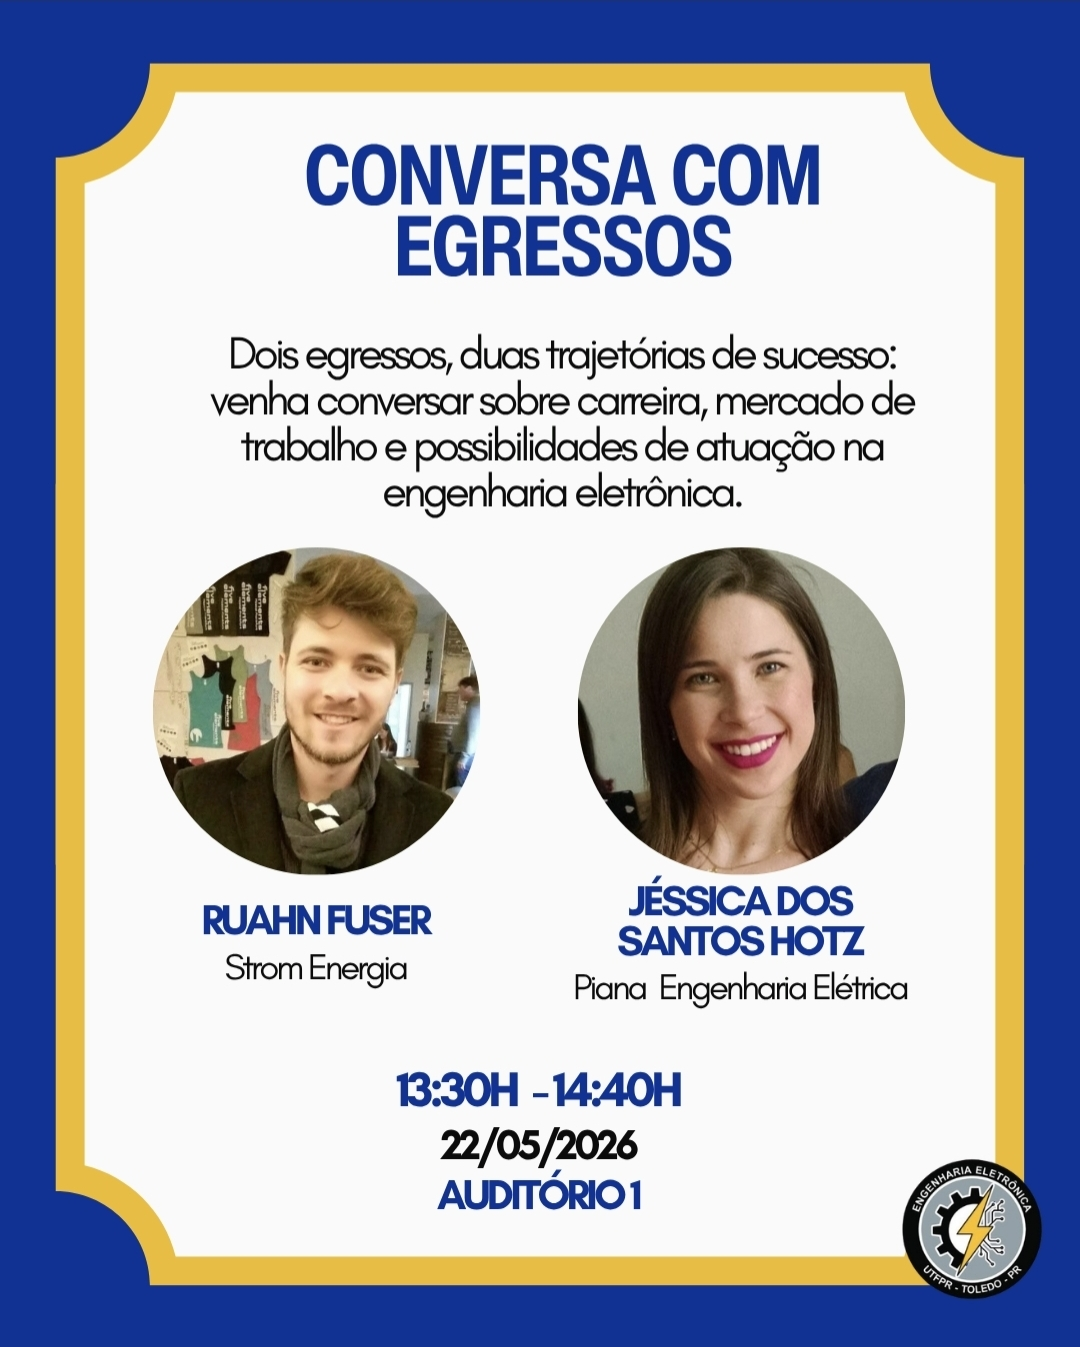
\includegraphics[width=0.56\textwidth]{img/Screenshot_20260522_123416_Samsung Internet.jpg}
    \caption{Material de divulgação da palestra ``Conversa com Egressos''.}
\end{figure}

\clearpage

\begin{figure}[H]
    \centering
    \begin{subfigure}{0.48\textwidth}
        \centering
        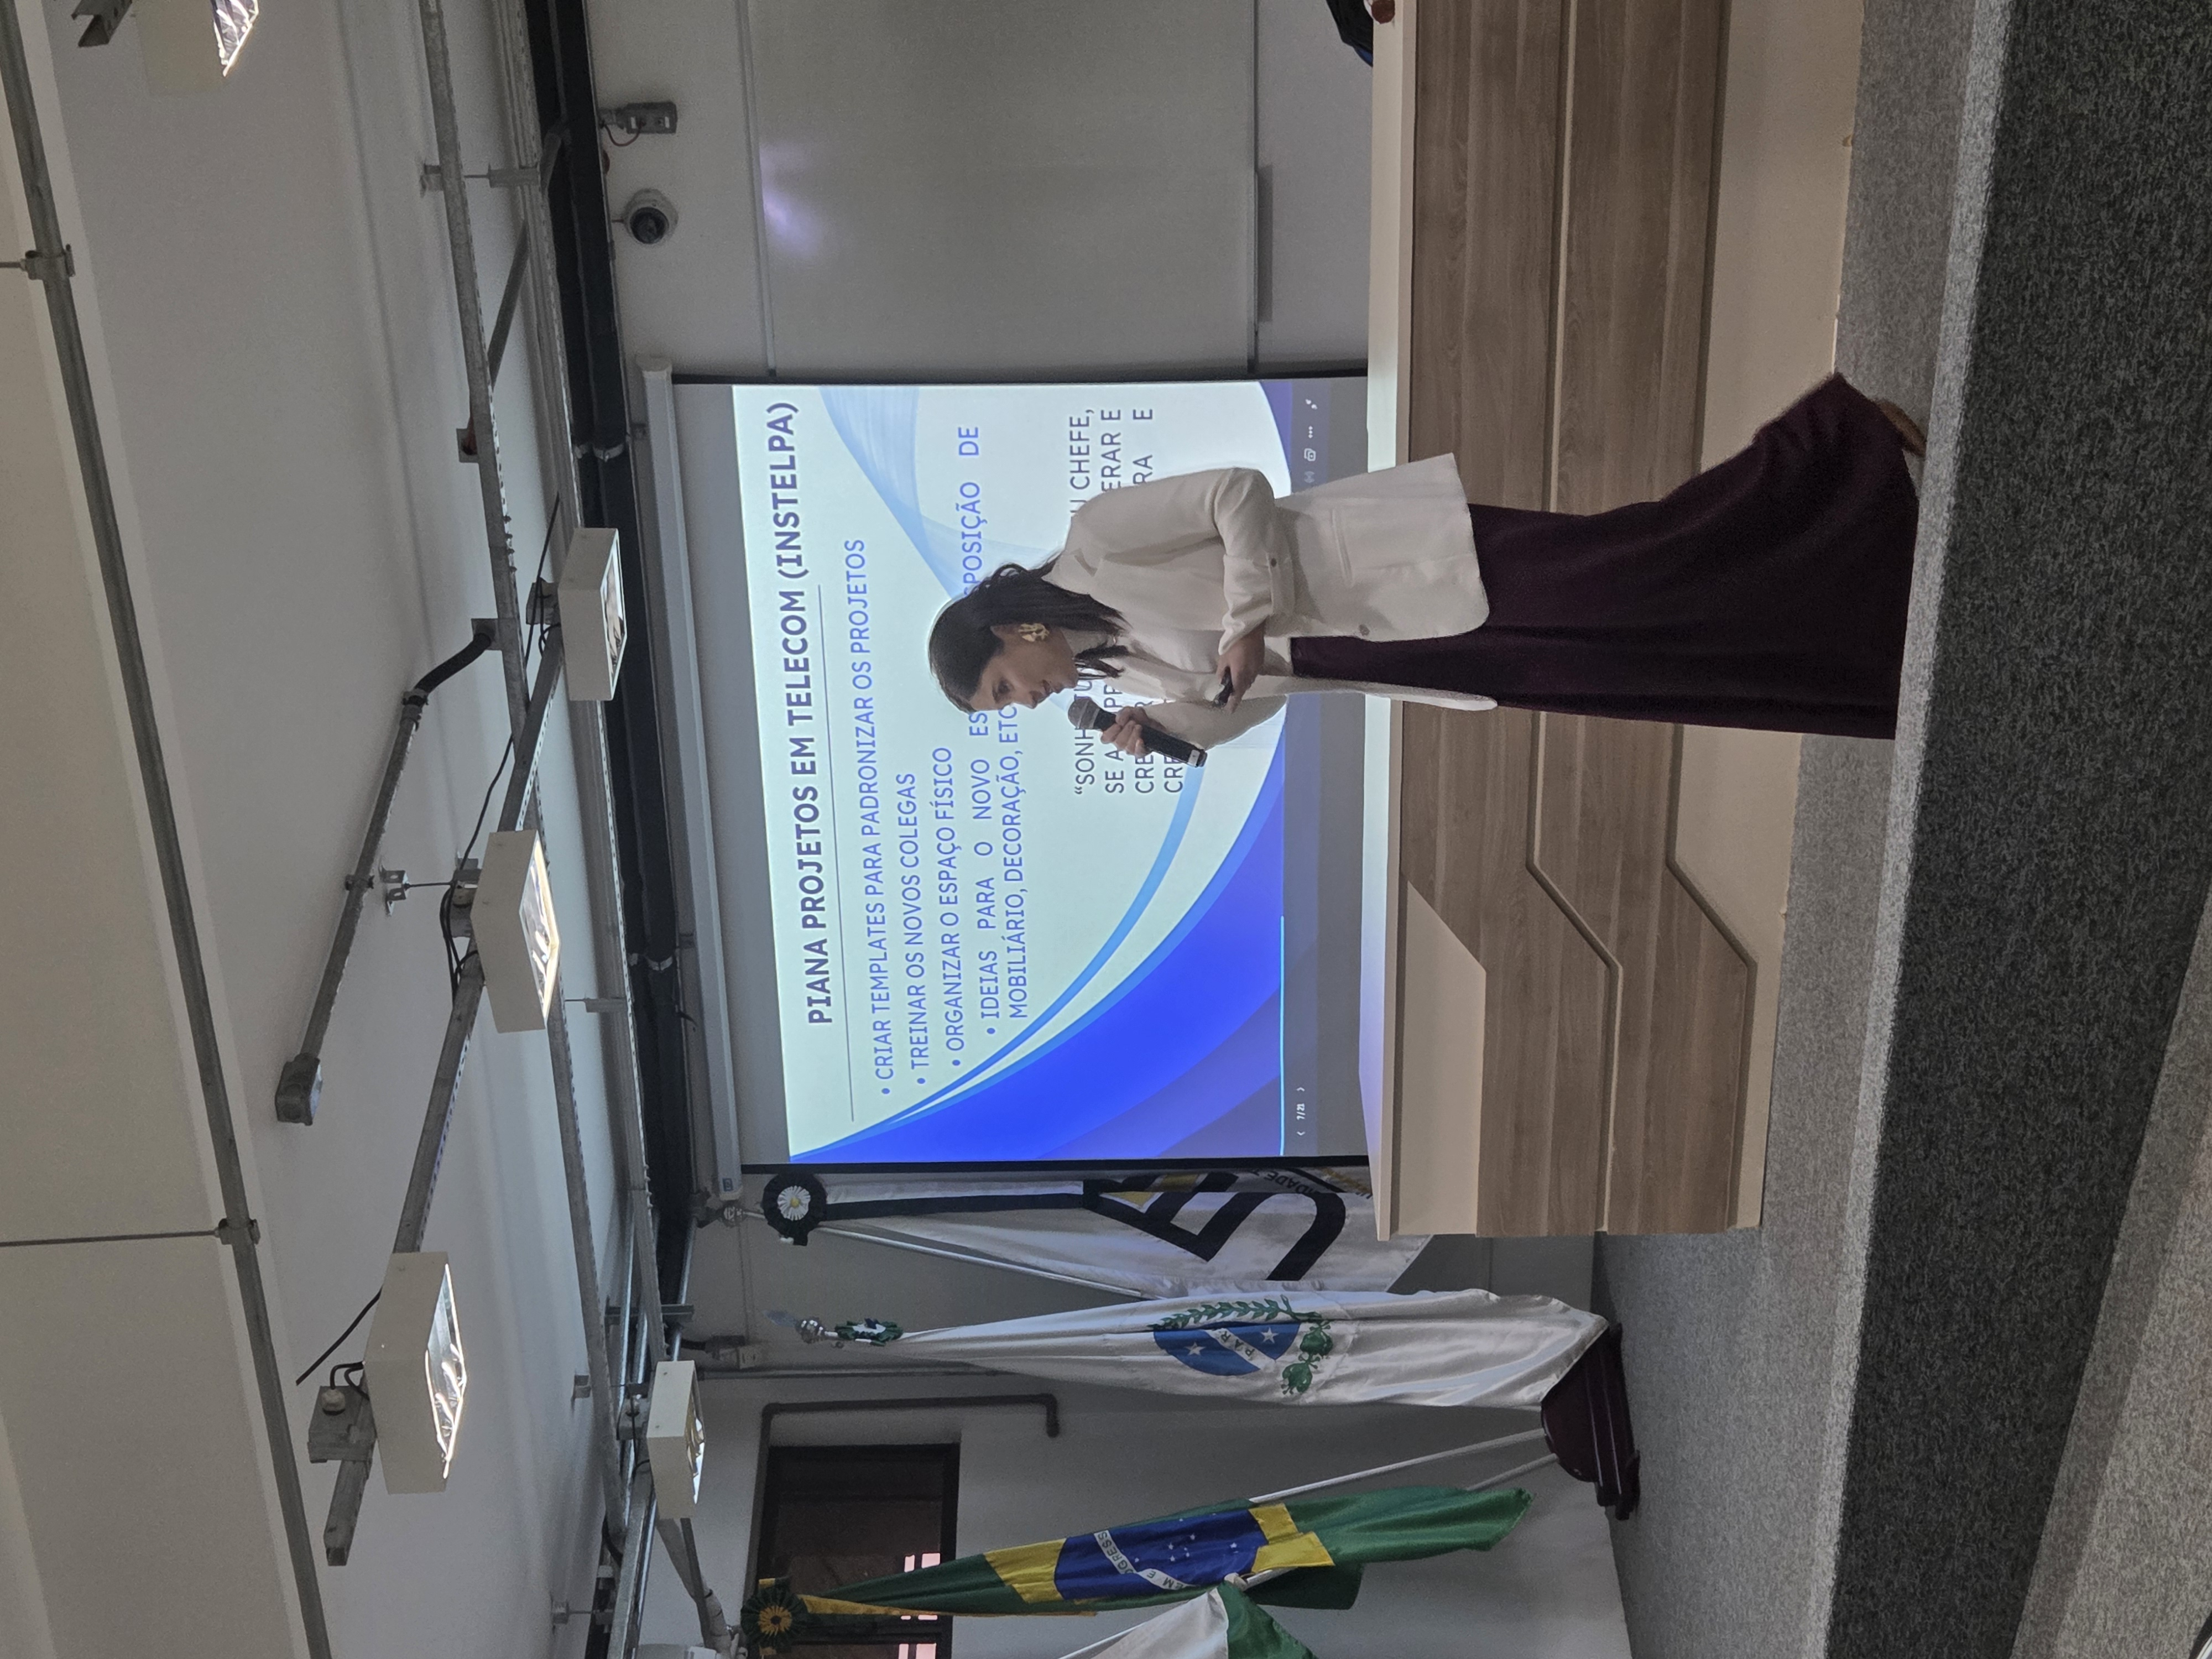
\includegraphics[width=\linewidth,angle=270]{img/20260522_134423.jpg}
        \caption{Apresentação de Jéssica dos Santos Hotz.}
    \end{subfigure}
    \hfill
    \begin{subfigure}{0.48\textwidth}
        \centering
        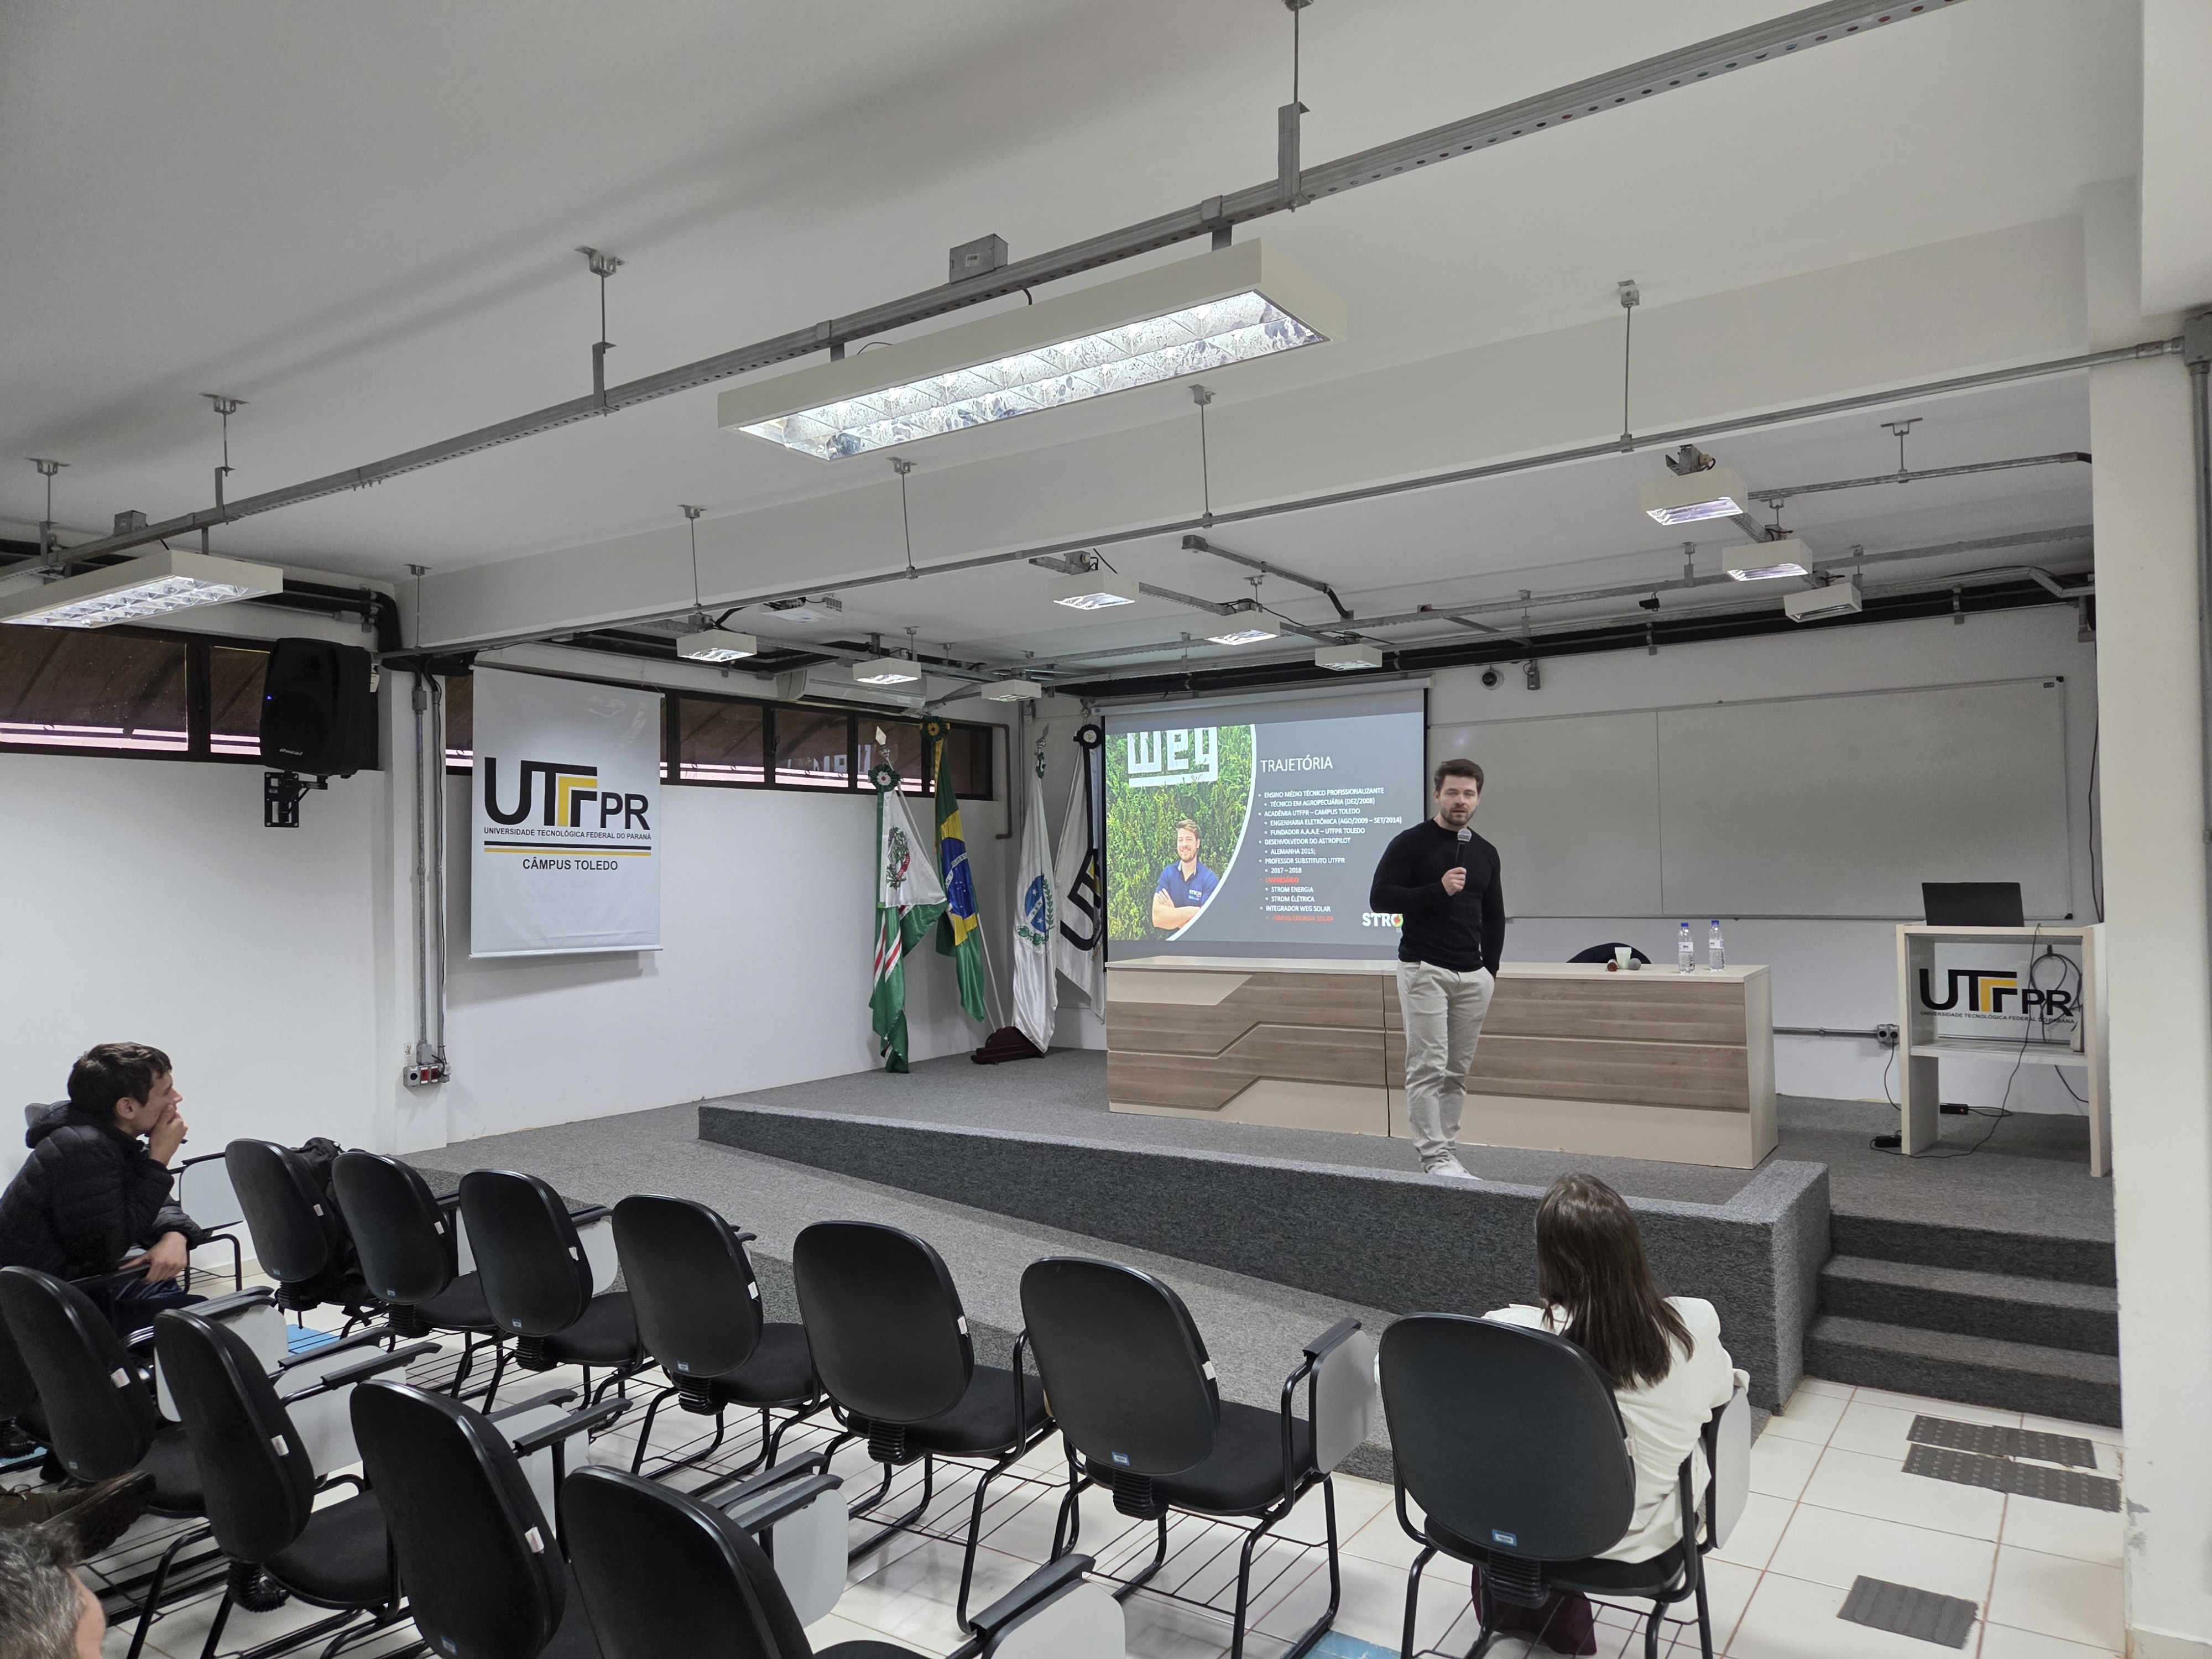
\includegraphics[width=\linewidth]{img/20260522_141516.jpg}
        \caption{Apresentação de Ruahn Fuser.}
    \end{subfigure}
    \caption{Participação dos egressos convidados no Auditório 1.}
\end{figure}

\begin{figure}[H]
    \centering
    \begin{subfigure}{0.48\textwidth}
        \centering
        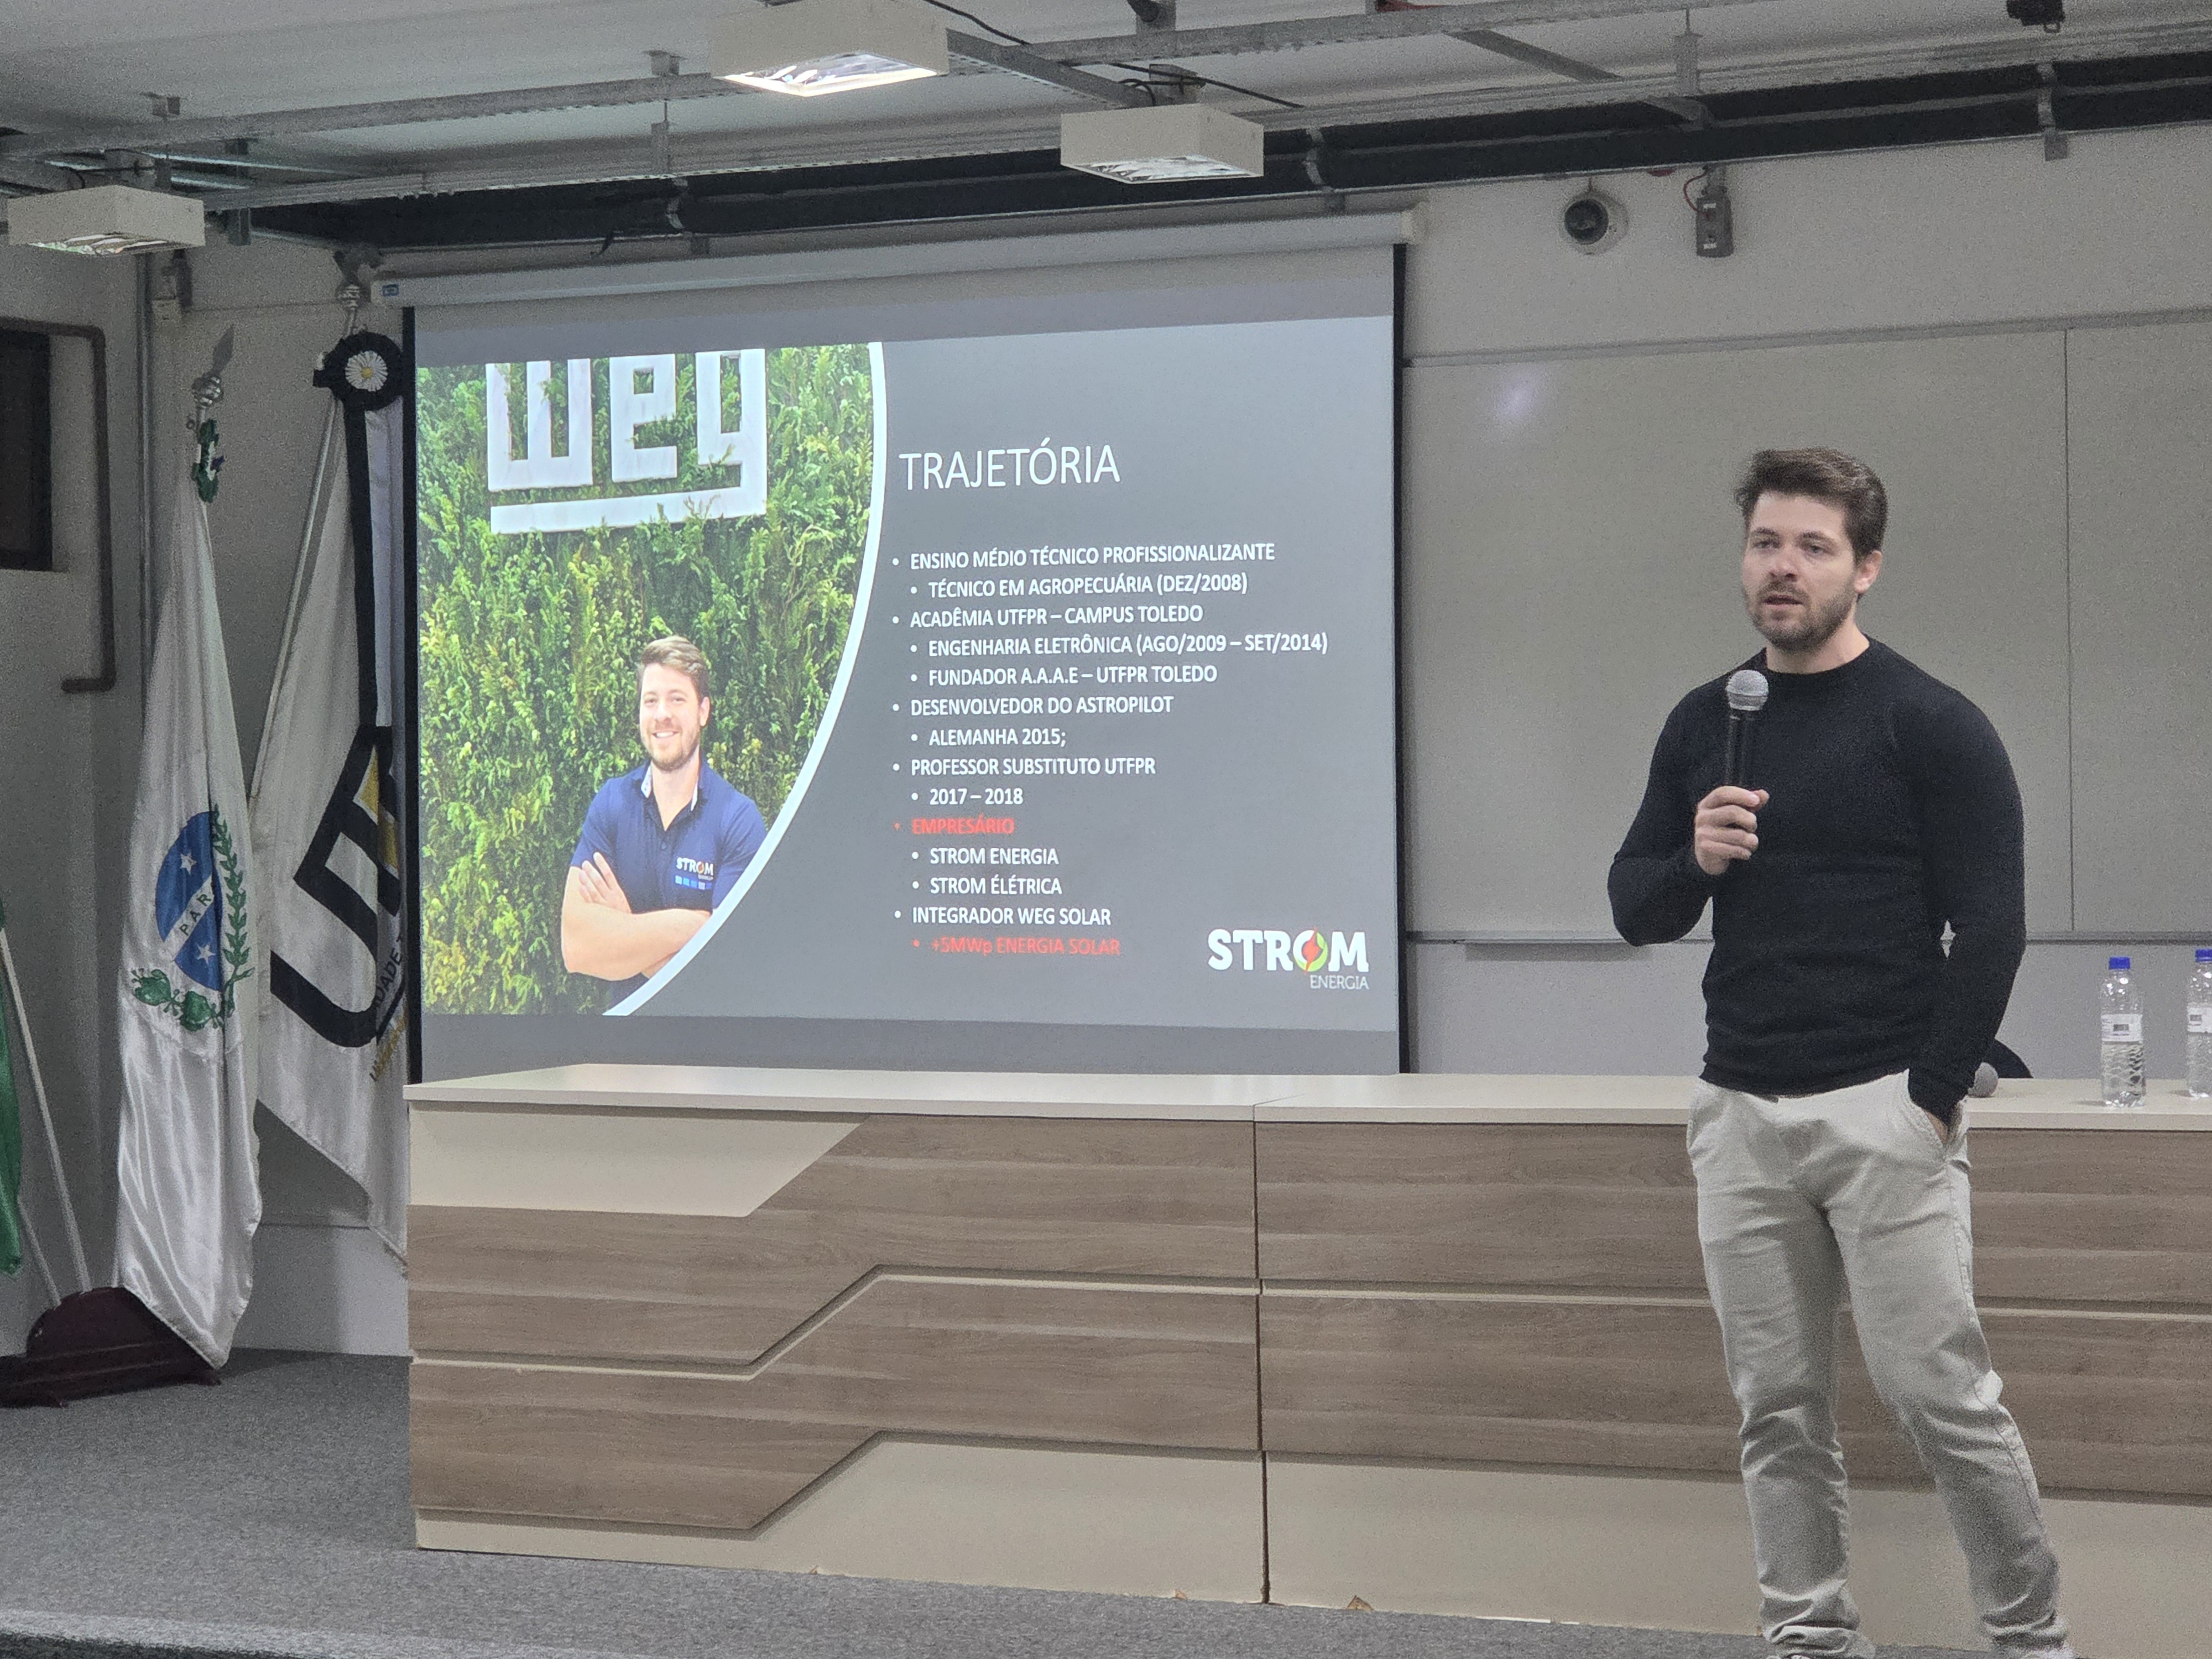
\includegraphics[width=\linewidth]{img/20260522_141520.jpg}
        \caption{Relato de trajetória profissional e experiência de mercado.}
    \end{subfigure}
    \hfill
    \begin{subfigure}{0.48\textwidth}
        \centering
        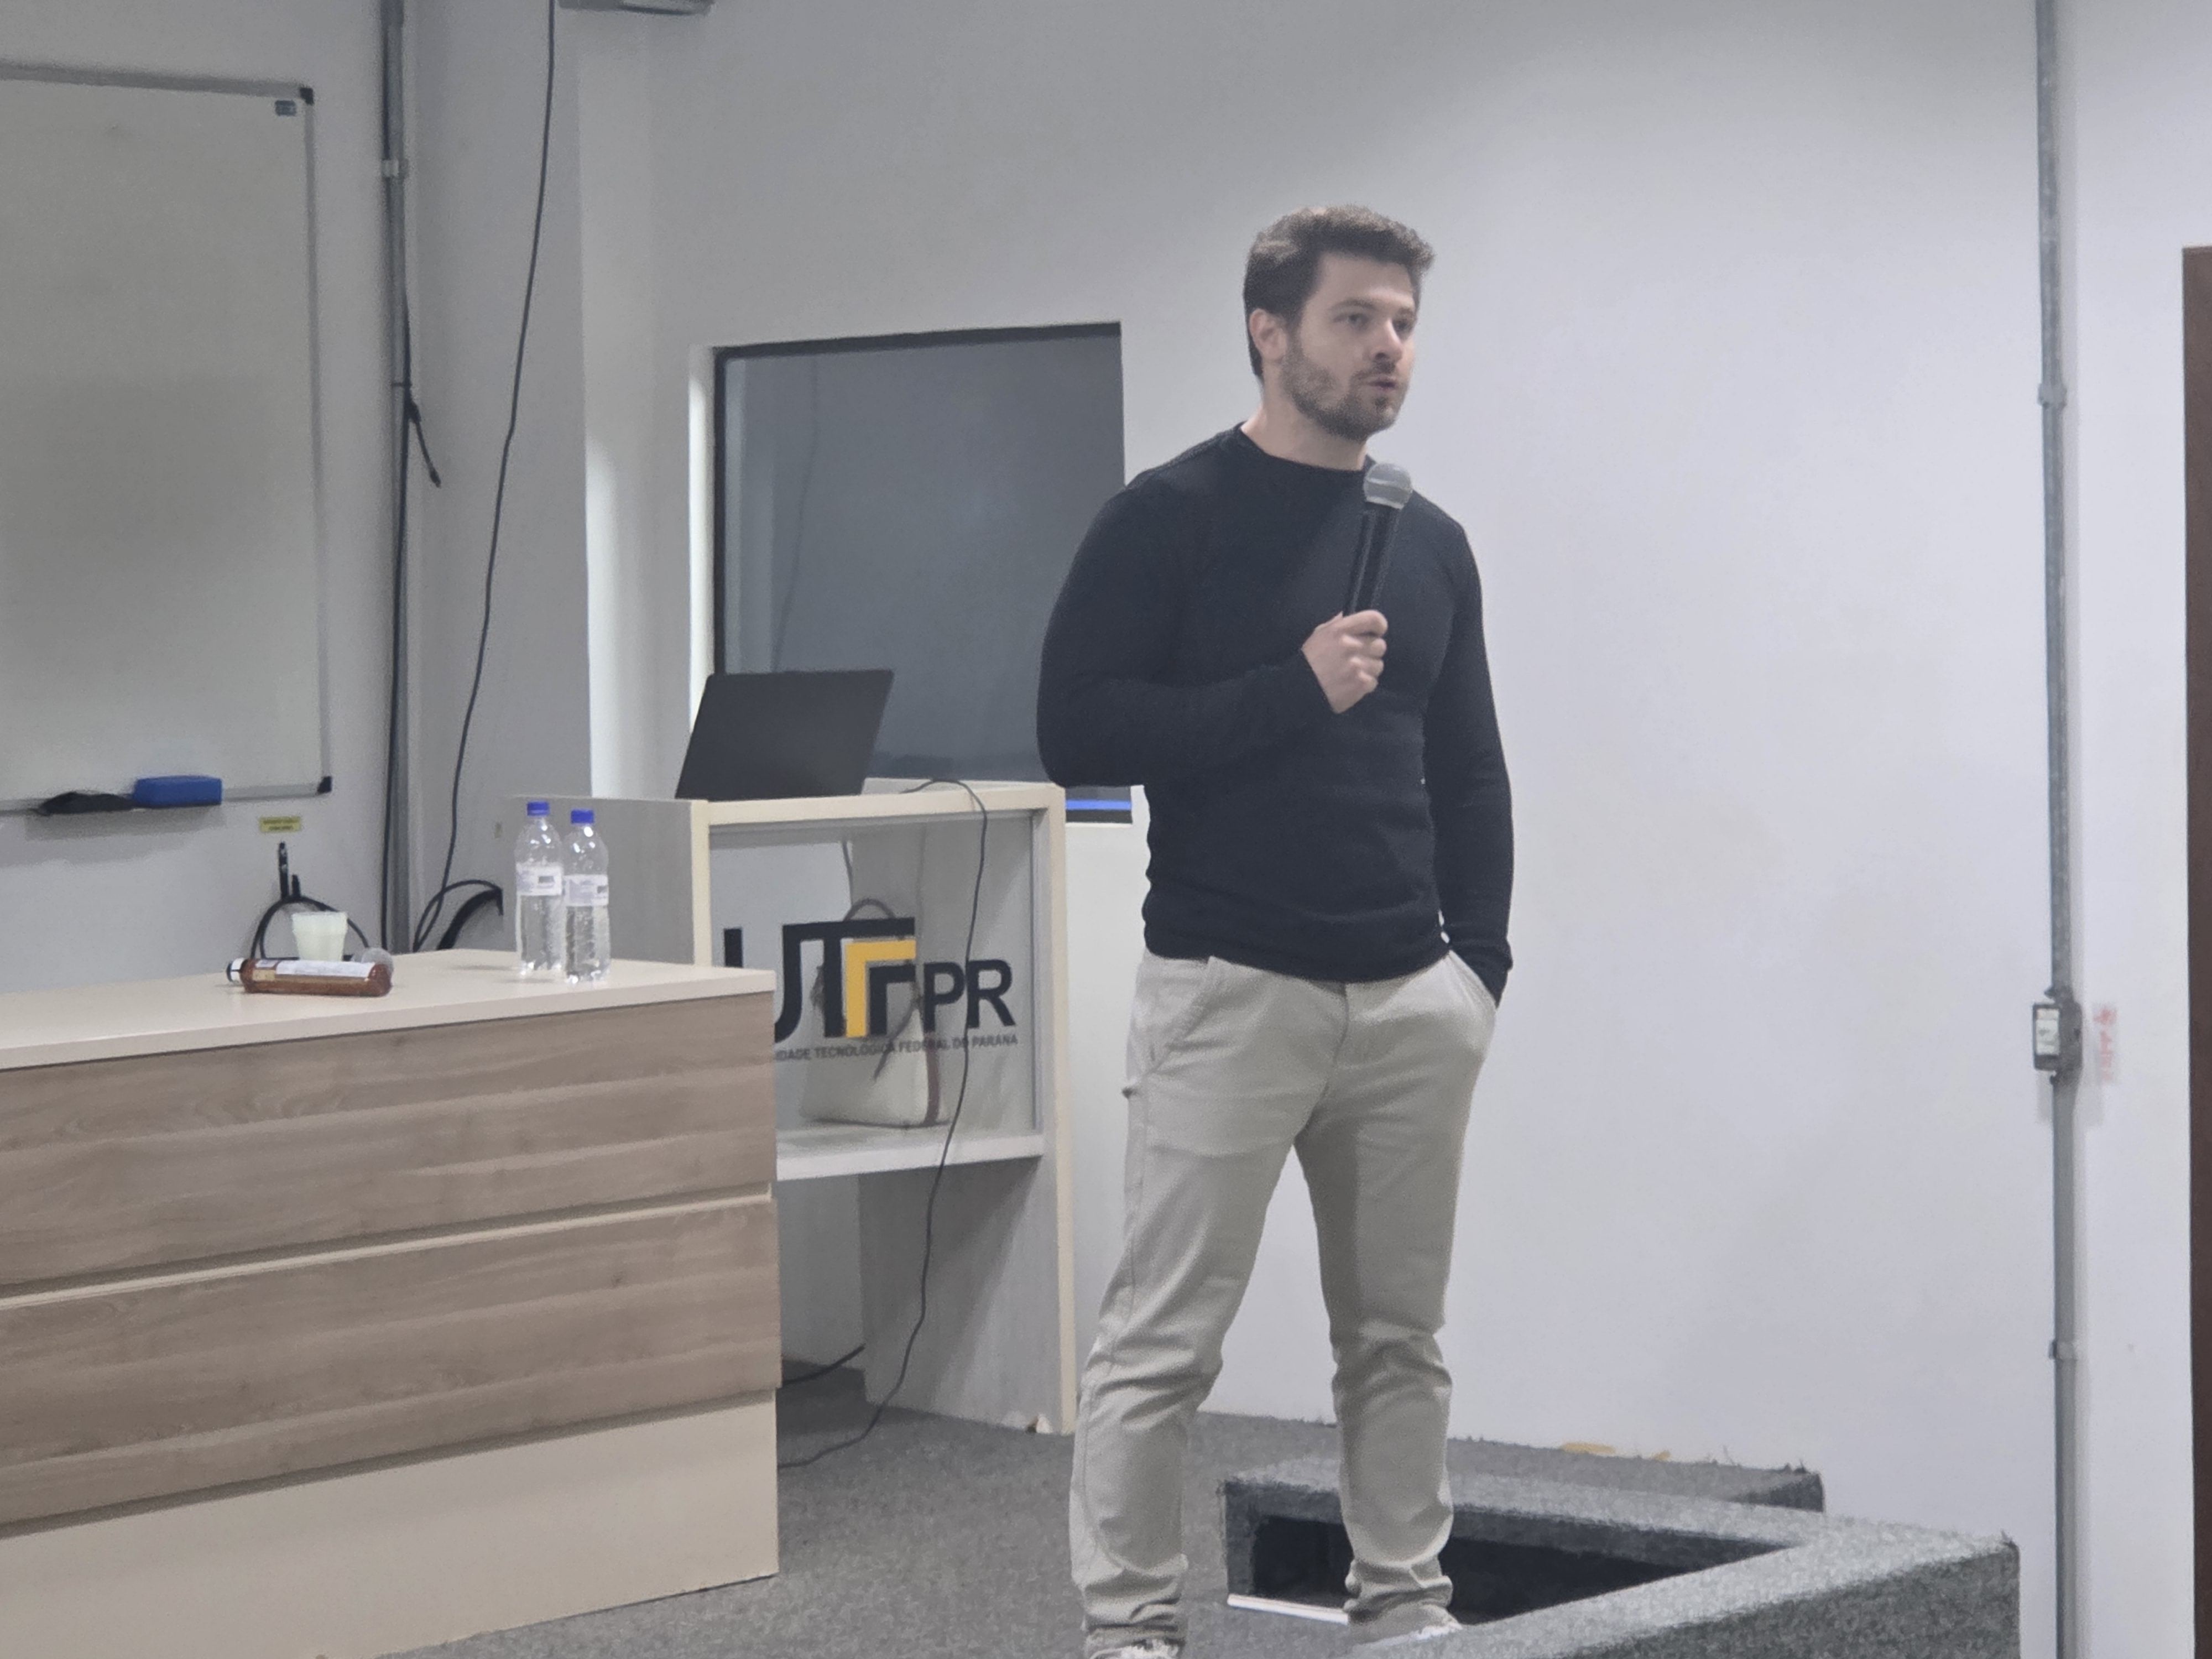
\includegraphics[width=\linewidth]{img/20260522_141600.jpg}
        \caption{Momento de interação com os participantes.}
    \end{subfigure}
    \caption{Registros da conversa com estudantes e demais participantes.}
\end{figure}

\end{document}
